\section{Method}
\label{sec:method}


\subsection{Parsing Rhythms}

We consider the observation of a rhythm to be a list of note onset times. In our system, note offsets are ignored. Although note offsets are rhythmically timed as well in many cases, note onsets seem to be the most important property of rhythms and also the property that rhythms played by any instruments have in common (it is hard for example to define the note offsets of a drum line). When note onsets are perceived as a rhythm, we assume that the perceived rhythm is an underlying structure. This structure defines a set of units, or metrical durations that form are the atomic units of the rhythm. These units are constrained to be duple or triple divisions of each other. Other prime number divisions are allowed as well but are far less common in Western music tradition. When a metrical unit is divided into two or three units, the leftmost unit is, by convention, called the downbeat. The other unit(s) are called upbeat(s).

A list of note onsets performed by a human is a noisy representation of the underlying structure. Some of this noise is caused by imperfection in the performance, some of the noise is caused by conscious deviation from the metronomic beat, otherwise known as expression.

The task of finding rhythmic structure can now be defined as finding the appropriate atomic units and finding the location of the downbeats. A structural representation of the rhythm should capture this information. Traditional staff notation is one possible structure that defines the location of downbeats and the atomic units that the onsets are build of. Instead of staff notation.

Every node in the subdivision tree represents a metrical duration. There are two types of terminals: an onset and a filler unit. A filler unit can be either a tied note or a rest. Since we are only looking at note onsets it does not make sense to distinguish tied notes from rests. The filler units will be referred to as ties from now on.

A node can be subdivided into any prime number of child nodes, although in this text we will assume that only duple and triple divisions are allowed. The metrical length of a node's child nodes is equal to the length of the node divided by the number of children. We do not need to define the length of the root node, and therefore metrical durations can be expressed relatively as a number of divisions of the root node. We can make a distinction between a \textit{metronomic duration} and a \textit{metrical duration}. Where a metronomic duration is a duration measured in some unit of time and a metrical duration is a duration relative to the root node. 

When humans perform a rhythm, some information about this underlying structure is encoded in the performance of the rhythm which may be why humans find it usually easy to hear the downbeat. In many music styles, it is common to emphasise the downbeat. It is hypothesised here that this emphasis takes the form of a slight asymmetry in the duration of the downbeat and the duration of the upbeat.

\subsubsection{Parser}

The goal of rhythmic parsing is to find a number of hypotheses about the underlying rhythmic structure of a list of note onsets. An hypothesis is formulated as a structural analysis, or subdivision tree. We assume that over a few notes, only a small number of hypotheses are likely. First, we present a parser that considers all possible hypotheses of a number of note onsets. After that, we present a method to select likely hypotheses and reject unlikely hypotheses. 

The parser is essentially a stochastic CKY parser that combines hypotheses about note onsets. It uses a small set of rules and two constraints that restrict it to form only valid rhythmic structures. 

\begin{align*}
\label{eq:rules}
D(\textsc{combine}([h_1, h_2])) &\rightarrow D(h_1) D(h_2)\\
D(\textsc{combine}([h_1, h_2, h_3)) &\rightarrow D(h_1) D(h_2) D((h_3)\\
D(h) &\rightarrow \textrm{On}_i\\
D(h) &\rightarrow *
\end{align*}
where $D(\phi)$ is a metrical duration with features $\phi$, $*$ represents a filler duration (this is needed when notes are tied together or when the first note is not the first beat of a measure) [SHOW SOME EXAMPLES HERE], $\textrm{On}_i$ is an onset at index $i$, $h$ is a hypothesis about the rhythmic analysis of the corresponding metrical duration and $\textrm{combine}/2$ and $\textrm{combine}/3$ are functions that take hypotheses and combine them into a new hypothesis.

The two constraints are:
\begin{enumerate}
\item Any set of two or three metrical durations are not allowed to combine if the first one expands directly to an onset and the others do not recursively expand to an onset.
\item Any set of two or three metrical durations is not allowed to combine if none of the recursively contains an onset.
\end{enumerate}

This parser is only constrained by the number of onsets in the input. In order to make it efficient it needs some way of rejecting unlikely hypotheses. The following section will explain this process.


\subsection{Hypothesis generation and rejection}
\label{sec:rejection}

[Rhythm, rhythmic analysis and hypothesis are used interchangeably here. Make some sense out of this]

The likelihood of a rhythm given a set of performed onsets is determined by two factors. One is how well the analysis matches the observed onset times and another is likely the rhythm itself is. [Picture of too detailed versus too simple analyses a la cemgil 2000]. In other words, we want to find the \textit{posterior} probability $P(A|N)$, where $A$ is a rhythm, and $N$ is a list of note onsets. We can formulate this as a generative model where

\begin{equation}
\label{eq:model}
P(A|N) \propto P(N|A)P(A).
\end{equation}

The posterior probability of a rhythm given a set of performed onsets is proportional to the probability that this rhythm generated the list of onsets, the \textit{likelihood} times the probability of the rhythm itself, the \textit{prior}.

Several authors have suggested that some rhythmic structures are more likely than others. \cite{cemgil2000rhythm} incorporated a notion of rhythmic complexity into their system for music transcription, where the likelihood of a rhythm is inversely proportional to its complexity. Temperley suggests a more thorough description of rhythm likelihood \citep{temperley2010modeling}. In \cite{temperley2009unified} he uses his hierarchical position model in a probabilistic music analysis system. [Explain somewhere why a PCFG captures Temperley's properties of common practice rhythm. If it even does...]. [Honing suggests a few priors somewhere else as well.]

Our hypotheses are represented as subdivision trees. This analysis suggests yet another way of characterising rhythm likelihood, commonly known as a probabilistic context-free grammar(PCFG). 

We will use several priors to evaluate our model. [these priors should be described in detail either here or in the evaluation section]

The likelihood should be a function that measures how well a hypothesis `fits' the observations. The simplest likelihood function is one that assigns zero probability to all hypotheses that do not exactly fit the observations. Such a likelihood would only allow metronomic performances. 

If we want to handle human performances we need to have tolerance for deviations from metronomic timing. In many models [citations], any deviation from metronomic timing is treated as additive noise. Deviations from metronomic timing are penalised using a normal distribution centred around the metronomic onset.

In order to define how our model determines the likelihood of an analysis, we first need to define how a subdivision tree implies metronomic onsets. 


\subsubsection{Combination}

Finding the onsets implied by an hypothesis is done in two steps. The first step is a bottom up process where as soon as enough onsets are available, the onset of downbeats containing ties are filled in. The second step is a top-down process where downbeat intervals are used to predict the location of upbeats. Since every downbeat except the first one is an upbeat at a higher level in our analysis, this process estimates the onsets of every onset in a piece.

For the first step, we need to extend our hypothesis representation to include onset times and the (estimated) downbeat onset. This is represented as a 3-tuple

\begin{equation}
h = (C, N, b_d)
\end{equation}

where $b_d$ is the downbeat, $N$ a list of onsets and $C$ is a list of child nodes. These child nodes are hypotheses themselves. A hypothesis thus defines a tree structure with onsets or ties as leaf nodes. A hypothesis is said to \textit{govern} a set of onsets if the hypothesis recursively contains these onsets. The number of children of a hypothesis defines its subdivision. In theory, a hypothesis can contain any prime number of child nodes, however in the explanation below we will limit this to the most frequent subdivisions of two and three.

A single onset is represented as $(\emptyset, [\textrm{on}], \textrm{on})$, where on is the onset time. A single tie is represented as $(\emptyset, [*], *)$.  Combining these hypotheses yields $([(\emptyset, [\textrm{on}], \textrm{on}), (\emptyset, [*], *)], [*, on], *)$. Generally, combining hypotheses can be described in the following manner: put the first element of the onset list $N$ of every subhypothesis in $N$ and, if the first element of the new $N$ is a tie, try to estimate the onset of the downbeat. If that is not possible or if the first element of $N$ is not a tie, set $b_d$ to the first element of $N$. Algorithm \ref{alg:combination} describes this process in detail.

When a hypothesis governs only one onset, the downbeat can not be estimated. Any hypothesis that does not contain an absolute or estimated downbeat is treated as a \textit{complex onset}. The hypothesis $(*$ $\bullet)$ for example is treated as an onset at relative position $0.5$, the hypothesis $(*$ $(*$ $\bullet))$ is treated as an onset with relative position 0.75.

[This explanation needs to be better and needs to contain examples]
The goal of the combination process is to get the best possible estimates of where the up and downbeats of a hypothesis are. The algorithm can be found in algorithm \ref{alg:combination}. The algorithm works roughly as follows. The input is a list $H$ containing two or three hypotheses. These will be the child nodes of the hypothesis that the combine function is building. The algorithm iterates through the list of hypotheses. If a hypothesis is an onset, the position of the onset and the absolute onset are added to \textit{onsets}. The position is a number between 0 and 2 or 0 and 3, depending on the number of hypotheses in $H$. If a hypothesis is a complex onset, its complex position, determined by the function \textsc{complexPostion}, and absolute onset are added to \textit{complexOnsets}. If a hypothesis suggests a downbeat, this downbeat and its position are added to \textit{onsets}.

\begin{algorithm}
\caption{Combine hypotheses}
\label{alg:combination}
\begin{algorithmic}
\Function{combine}{$H$}
	\State $d \leftarrow$ \Call{length}{$H$}
	\Comment{Division}
	\State onsets $\leftarrow \emptyset$
	\State complexOnsets $\leftarrow \emptyset$
	\State $N \leftarrow \emptyset$
	\State $C \leftarrow H$
	\For{$i \leftarrow 0,d$}
		\State $(C', N', b_d') \leftarrow H[i]$
		\If{$C = \emptyset$ \textbf{and} $N \neq [*]$}
			\State \textbf{append} ($i, H[i]$) \textbf{to} onsets
		\Else
			\If{$b_d' \neq *$}
			\Comment{Check if the hypothesis suggests a downbeat}
				\State \textbf{append} $(i, b_d')$ \textbf{to} onsets
			\Else
				\State $p$, complexOnset $\leftarrow$ \Call{complexPosition}{$H[i]$}
				\State \textbf{append} ($i + p$, complexOnset) \textbf{to} complexOnsets
			\EndIf
		\EndIf
	\EndFor
	\If{\Call{length}{onsets} $\leq 1$}
		\State \textbf{append} complexOnsets \textbf{to} onsets
	\EndIf
	\State $b_d \leftarrow N[0]$
	\If{$b_d = *$}
		\State $b_d \leftarrow$ \Call{downbeat}{onsets, $d$}
	\EndIf
	\State \textbf{return} $(C, N)$
\EndFunction
\end{algorithmic}
\end{algorithm}

Once the algorithm has iterated thought $H$, the algorithm checks whether there is an onset on the downbeat. If there is not, the \textsc{downbeat} function attempts to estimate the downbeat from the list of onsets. We assume that an interval based on one or more complex positions is less reliable than an interval based on intervals between downbeats. Only if \textit{onsets} contains less than two onsets, \textit{complexOnsets} is added to it. When the combined length of \textit{onsets} and \textit{complexOnsets} is 1, this hypothesis governs only one onset and the list of beats will only contain that onset and one or more ties. If the combined \textit{onsets} and \textit{complexOnsets} contains more than one onset, the \textsc{downbeat} function estimates downbeat from these onsets

In a practical implementation, every hypothesis should also keep track of the first onset before and after the hypothesis. This can be used later to restrict endlessly adding ties to the hypothesis. [More explanation]

\subsubsection{Observations}

The combination process combines hypotheses makes sure that every hypothesis governing more than one note contains an estimated downbeat. The observations function uses this information to transform a hypothesis into a list of features that define how likely a hypothesis is given the absolute onsets that it governs. The observations function should clearly discriminate between unlikely interpretations and likely interpretations of an onset pattern. [Example of likely and unlikely hypotheses here].

The observation function is a top-down recursive function. It calculates the expected onset of every down- and upbeat of every hypothesis in the tree. The main assumption of the function is that the expected onsets of the upbeats at level some are derived from the downbeat interval at the level above. 

For a hypothesis $h = (C, N, b_d)$, the algorithm is initialised as follows: $\textsc{observations}(h, b_d, *, \textsc{length}(C) \times (N[1] - b_d))$, where $\textsc{length}(C) \times (N[1] - b_d)$ is the division times the length interval of the downbeat and the first upbeat.
\begin{algorithm}
\caption{Generate observations}
\label{alg:observations}
\begin{algorithmic}
\Function{observations}{$h$, downbeat, nextDownbeat, estimatedDownbeat}
	\If {downbeat $ = *$}
		\State \textbf{return} $\emptyset$
	\EndIf
	\State $C, N, d_b \leftarrow h$
	\If {$b_d \neq *$}
		\Comment{If this $h$ implies a downbeat, use it.}
		\State downbeat $\leftarrow d_b$
	\EndIf
	\If {nextDownbeat $ = *$}
		\State nextDownbeat $\leftarrow$ estimatedDownbeat
	\EndIf
	\State \textbf{append} nextDownbeat \textbf{to} $N$
	\State $d \leftarrow$ \Call{length}{$C$}
	\Comment{Division of this $h$.}
	\State $l \leftarrow$ nextDownbeat - downbeat
	\Comment{The estimated length of this $h$.}
	\State $O \leftarrow \emptyset$
	\Comment{Observations.}

	\For {$i \leftarrow 1,d$}
		\If {$N[i] \neq *$ \textbf{and} $i \neq 0$}
			\State \textbf{append} \Call{$\Phi$}{downbeat, nextDownbeat, $B[i]$, $i$, $d$} \textbf{to} $O$
		\EndIf	
		\State $C', N', b_d' \leftarrow C[i]$
		\If {$C' \neq \emptyset$}
			\State $b_{\mathrm{down}'} \leftarrow \mathrm{downbeat} + l * i/d$
			\If {$N'[i] \neq *$}
				\State $b_{\mathrm{down}} \leftarrow B[i]$
			\EndIf
			\State $b_{\mathrm{up}} \leftarrow b_{\mathrm{down}} + l/d$
			%\If{$B[i+1] \neq *$}
			%	\State upbeat $\leftarrow B[i+1]$
			%\EndIf
			\State \textbf{append} \Call{observations}{$(C', B'), b_{\mathrm{down}}, b_{\mathrm{up}}$} \textbf{to} O
		\EndIf
	\EndFor
	\State \textbf{return} O
\EndFunction
\end{algorithmic}
\end{algorithm}

Given an expected and observed onset

Any machine learning algorithm can be used to learn a mapping from features to ratio. This makes the model suitable for a rhythmic-structure-aware expressive timing model.


\begin{equation}
\Phi(\beta, \beta', b, i, d) = \frac{(b - \beta) / i}{(\beta' - b) / (d - i)},
\end{equation}
where $\beta$ is a downbeat, $\beta'$ is the next downbeat, $b$ is an onset, $i$ is the position of $b$, and $d$ is the number of beats between $\beta$ and $\beta'$ (the division).

Calculating likelihood

We can now calculate the likelihood of any hypothesis by taking the product of the observations that it implies. Optionally we can add an expression parameter that suggests the ratios to be slightly larger than one. The (normalised) likelihood of a set of observations is

\begin{equation}
\label{eq:h_likelihood}
\mathcal{L}(O|h, \mu, \sigma) \propto \prod_{i=0}^N \exp\left(-\frac{(\mu - \log(O_i))^2}{2\sigma^2}\right)
\end{equation}

Where $O$ is a set of down-/upbeat ratios. We expect the down-/upbeat ratios to be close to one and their to be logarithm close to zero. Therefore it makes sense to set $\mu$ to zero. However we may expect downbeats to be slightly stretched and we can set $\mu$ to reflect this.

Rejecting hypotheses

A hypothesis is rejected if the per item likelihood is lower than a certain threshold. The per-observation likelihood is defined as

\begin{equation}
\label{eq:per_obs_likelihood}
\mathcal{L}(O|h, \mu, \sigma) \mbox{ per observation } \propto \exp\left(-\frac{1}{N}\sum_{i=0}^N \frac{(\mu - \log(O_i))^2}{2\sigma^2}\right)
\end{equation}


%Constraints of the corpusparser (a parser that only allows metronomic performances)

%Single note analysis constraints

%Constraint in adding ties


%Introducing triple divisions introduces ambiguities between triple divisions or more complicated constructions of duple divisions (that are quite unlikely).

%For this we extend the duration symbol with three optional features. Every symbol now has a vector of onsets or ties. The first item of this vector is defined to be the downbeat, the rest are upbeats. The interval of the downbeat and the first upbeat at level $l$ is the downbeat interval at level $l+1$. This notion is the basis of the model. As soon as a vector contains more than one onset, the vector is filled in with expected onsets given the two onsets.


\subsection{Data Preparation}

The parser's likelihood function takes two parameters: an expected logarithmic down-/upbeat ratio and its standard deviation. To estimate these values, a corpus of amateur jazz performances was prepared.

The corpus contains Jazz and Latin standards that were scraped off the the web [Cite Mark GW?]. The performances are generally of good quality and are played in a relatively constant tempo. In its original form, the corpus was a set of multi-track MIDI files containing both tracks played by a human performer and tracks generated by a computer in metronomic time.

MIDI files represent music as a list of note-on and note-off events, corresponding to key presses and key releases. Every event has the parameters pitch, velocity and delta-time. Delta-time specifies the time between this events and the last one, pitch is the pitch of the key that was pressed, velocity is the velocity with which the key was pressed or released.

For our purposes we want to have monophonic melody tracks played by a human performer. To get these tracks, every file in the corpus was split into separate tracks. Monophonic tracks played by humans were filtered out automatically. This was done by assuming that tracks played by humans contained a lot of variation in onset velocity and in inter-onset intervals due to imperfect timing. From this subset of performed tracks, tracks containing melodies where selected by hand. 

After the filtering process, [N-CORPUS] tracks were left containing melodies of [N-STANDARDS] different standards. These MIDI files where converted to note lists of the following format

\begin{align*}
N &= \{n_0, n_1, \cdots, n_N\},\\
n_i &= (\mathrm{On}_i, \mathrm{Pitch}_i, \mathrm{Velocity}_i),
\end{align*}
where $N$ is a note list containing notes $n_0$ to $n_N$. A very simple annotation format was chosen: every note in the note list was annotated with its metrical position, measured in quarter notes. 

Most of the corpus was played in swing, were it is common to play upbeat eighth notes as slightly delayed so that they fall on the third note of a eigth note triple, in terms of subdivision, the third beat of a quarter note divided by three. The example in figure \ref{fig:swing:a} shows a rhythm with some upbeat eighth notes. When performed in swing, the performance is usually closer to figure \ref{fig:swing:b}.

Although we now have metrical onsets, we still do not have the subdivision trees for the corpus. A simple parser with a flat prior and likelihood function that only allowed metronomic timing was used to generate parses for every item in the corpus. From these results correct parses where selected by hand. A subdivision tree for the swing example is shown in figure \ref{fig:swing:c}.


\begin{figure}
\centering
\subfloat[Rhythm notation]{
\label{fig:swing:a}
\centering
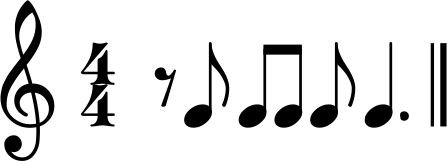
\includegraphics[scale=0.3]{img/aint_misbehavin}
}
\\
\subfloat[Annotation]{
\label{fig:swing:b}
\centering
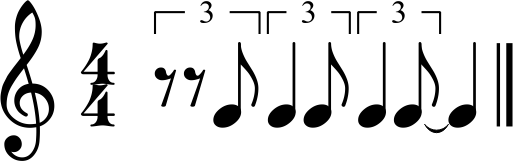
\includegraphics[scale=0.3]{img/aint_misbehavin_swung}
}
\\
\subfloat[Parsetree]{
\label{fig:swing:c}
\centering
\Tree 
[ .{$\frac{1}{1}$} [ .{$\frac{1}{2}$} [ .{$\frac{1}{4}$} [ .$*$ ] [ .$*$ ] [ .$\bullet$ ] ] [ .{$\frac{1}{4}$} [ .$\bullet$ ] [ .$*$ ] [ .$\bullet$ ] ] ] [ .{$\frac{1}{2}$} [ .{$\frac{1}{4}$} [ .$\bullet$ ] [ .$*$ ] [ .$\bullet$ ] ] [ .$*$ ] ] ]
}
\caption{Annotation of swung notes.}
\end{figure}

\subsection{Training}

\subsubsection{Prior}

The prior should be an indication of how likely a rhythmic analysis is a priori. If the likelihood would be the only indication of the quality of an analysis, the analysis would become too detailed like in figure \ref{fig:detailed}. A prior is needed to prefer sensible analyses and reject over complicated ones. In addition to that, without a prior, the model would have no way of determining the phase (the location of the downbeats). [give example of equally likely analyses with different phases but more unlikely priors]

The prior used in this study is simply a probabilistic context-free grammar (PCFG). Usually, a PCFG assigns probabilities to the expanding of a non-terminal symbol to other non-terminal symbols. In our case, probabilities of non-terminal symbols to terminal symbols are included as well since there are only two terminal symbols.

The only non-terminal symbol in our grammar is a hypothesis that has child nodes. There are two terminal symbols: an onset and a tie. Since there is only one non-terminal in the grammar, the probability that a hypothesis $h$ expands to child nodes $C$ is given by

\begin{equation}
P((C, N, b_d) \rightarrow C) = P((C, N, b_d)) = \frac{\mathrm{count}((C, N, b_d))}{N},
\end{equation}
where N is the total number of non-terminal symbols.

\subsubsection{Expression model}

$\mu$ and $\sigma$ for the bottom 4 levels?


\subsection{Parser optimisations}

To make the parser computationally tractable, a few optimisations were needed. It was already mentioned that the parser uses a beam parameter to reject unlikely hypotheses. In addition to that a few extra measures had to be taken.

First of all, the \textsc{observations} function returns no observations for hypotheses containing a single onset (complex onsets). Their probability is always one and theoretically ties could be added endlessly. To restrict this the parser maintains a small list of allowed single note analyses. This list is compiled by taking all single-note analyses found in the labelled corpus.

Second of all, the corpus contains only 4/4 time signatures, therefore triple divisions are allowed only at note level. All allowed triple divisions are shown in figure \ref{fig:triples}. 

\begin{figure}
$\bullet$
\Tree
[ .{$\frac{1}{1}$} [ .$*$ ] [ .$\bullet$ ] ] 
\Tree
[ .{$\frac{1}{1}$} [ .$*$ ] [ .$*$ ] [ .$\bullet$ ] ] 
\Tree
[ .{$\frac{1}{1}$} [ .$*$ ] [ .{$\frac{1}{2}$} [ .$*$ ] [ .$\bullet$ ] ] ] 
\Tree
[ .{$\frac{1}{1}$} [ .$*$ ] [ .{$\frac{1}{2}$} [ .{$\frac{1}{4}$} [ .$*$ ] [ .$\bullet$ ] ] [ .$*$ ] ] ] 
\caption{Some single note analyses.}
\label{fig:singlenotes}
\end{figure}

\begin{figure}
\Tree
[ .{$\frac{1}{1}$} [ .$*$ ] [ .$*$ ] [ .$\bullet$ ] ] 
\Tree
[ .{$\frac{1}{1}$} [ .$\bullet$ ] [ .$*$ ] [ .$\bullet$ ] ]
\Tree 
[ .{$\frac{1}{1}$} [ .$\bullet$ ] [ .$\bullet$ ] [ .$\bullet$ ] ]
\caption{Allowed triple divisions.}
\label{fig:triples}
\end{figure}

Third of all, the parser may at some point generate a large number of hypotheses due to ambiguities in the input. We do not need to keep track of all those hypotheses because the prior is able to select the most likely ones. The parser therefore only includes the best-$n$ hypotheses in every cell, where hypotheses are ranked by their posterior probability.
% Beam
% Triple divisions
% Best-n
% Max depth
%

\subsection{Overview}

% Chart parsing, beam, prior, likelihood, 
